\begin{physicsnote}{מנהלות: סוף הקורס והמבחן}
השיעור היום הוא האחרון שמועבר על ידי המרצה (בצלאל יחליף בשיעור הבא).
לגבי המבחן:
\begin{itemize}
    \item \textbf{חומר עזר:} יסופקו 4 דפי נוסחאות, מותר להביא עד 10 דפים אישיים (ניתן להעלותם לבדיקה מראש).
    \item \textbf{מבנה:} ככל הנראה 3 או 4 שאלות (ללא בחירה, כדי לשמור על הוגנות).
    \item \textbf{אופי השאלות:} שאלה ראשונה ושנייה לרוב עוסקת בהוכחות או טענות כלליות (למשל: עקרון הווריאציה). שאר השאלות יצריכו חשיבה ויישום.
    \item \textbf{המלצה ללמידה:} לפתור תרגילים לבד (משלב הקריאה ועד הפתרון הסופי) ללא הצצה בפתרונות, כדי לפתח "כושר" פתרון בעיות.
\end{itemize}
\end{physicsnote}


\section*{הרצאה: מבוא לתורת הפיזור (\LR{Scattering Theory})}

\subsection*{1. רכיבי הניסוי והנחות יסוד}
תהליך הפיזור בפיזיקה קוונטית הוא הכלי המרכזי לחקירת מבנה החומר ואינטראקציות מיקרוסקופיות. הניסוי מורכב משלושה רכיבים עיקריים:
\begin{itemize}
    \item \textbf{\LR{Projectile} (קליע):} חלקיק הנורה ממקור (מאיץ) לעבר המטרה. נתאר אותו כחבילת גלים צרה מאוד בתנע, השקולה בקירוב לגל מישורי (\LR{Plane Wave}).
    \item \textbf{\LR{Target} (מטרה):} פוטנציאל המפזר את החלקיק הנכנס.
    \item \textbf{\LR{Detector} (גלאי):} ממוקם במרחק מאקרוסקופי מהמטרה ומודד את החלקיקים שהתפזרו בזוויות שונות.
\end{itemize}

\begin{definitionbox}{הנחות המודל הסינתטי}
בדיון זה נניח את ההנחות הבאות:
\begin{enumerate}
    \item הקליע חסר מבנה פנימי וחסר ספין (\LR{Spinless}).
    \item המטרה מתוארת על ידי פוטנציאל מפזר $V(\vec{r})$.
    \item הקינמטיקה אינה יחסותית.
    \item הפוטנציאל הוא \textbf{קצר טווח}: $V(r) \approx 0$ עבור $r > R$ (כאשר $R$ הוא רדיוס מיקרוסקופי). הנחה זו מוציאה מכלל דיון את פוטנציאל קולון (\LR{Coulomb Potential}), הדורש טיפול מיוחד בשל טווחו האינסופי.
\end{enumerate}
\end{definitionbox}

\begin{center}
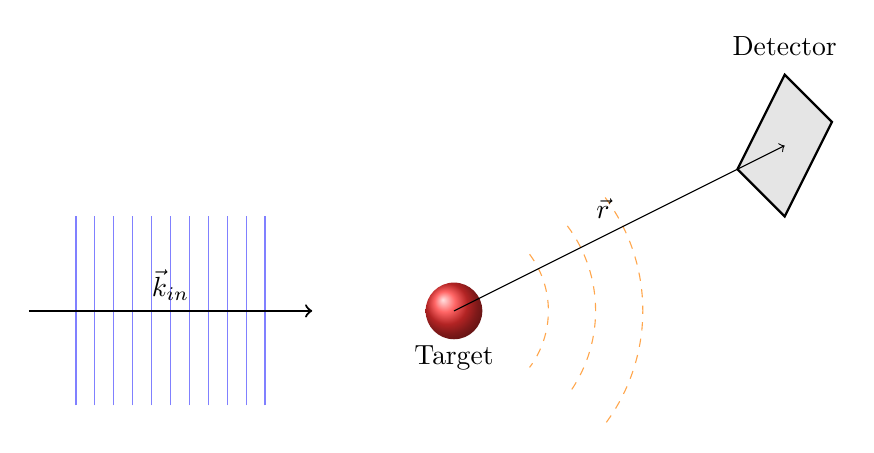
\begin{tikzpicture}[scale=1.2]
    % Incoming wave
    \foreach \x in {-4,-3.8,...,-2}
        \draw[blue!50] (\x,-1) -- (\x,1);
    \draw[->, thick] (-4.5,0) -- (-1.5,0) node[midway, above] {$\vec{k}_{in}$};
    
    % Target
    \shade[ball color=red!80] (0,0) circle (0.3);
    \node at (0,-0.5) {\LR{Target}};
    
    % Scattered waves
    \foreach \r in {1,1.5,2}
        \draw[orange!70, dashed] (\r*0.8, \r*0.6) arc (36.8: -36.8: \r);
    
    % Detector
    \draw[thick, fill=gray!20] (3,1.5) -- (3.5,2.5) -- (4,2) -- (3.5,1) -- cycle;
    \node at (3.5,2.8) {\LR{Detector}};
    \draw[->] (0,0) -- (3.5,1.75) node[midway, above left] {$\vec{r}$};
\end{tikzpicture}
\end{center}

\subsection*{2. חתך פעולה ואמפליטודת פיזור}
הגודל הפיזיקלי הנמדד בניסוי הוא \textbf{חתך הפעולה הדיפרנציאלי} (\LR{Differential Cross-Section}), המוגדר כקצב האירועים ליחידת זמן חלקי השטף הנכנס:
$$\frac{d\sigma}{d\Omega} = \frac{1}{J_{inc}} \frac{dN}{d\Omega}$$

נניח גל נכנס מהצורה:
$$\phi_{inc}(\vec{r}) = \frac{1}{\sqrt{\mathcal{V}}} e^{i\vec{k}\cdot\vec{r}}$$
כאשר $\mathcal{V}$ הוא נפח העולם. שטף ההסתברות הנכנס (\LR{Incident Flux}) מחושב לפי:
$$\vec{J}_{inc} = \frac{\hbar}{m} \text{Im}(\phi^* \nabla \phi) = \frac{\hbar k}{m \mathcal{V}} = \frac{v}{\mathcal{V}}$$

רחוק מהמטרה ($r \to \infty$), פונקציית הגל המפוזרת צריכה להתנהג כגל כדורי יוצא:

\[H=\frac{P^2}{2m}=-\frac{\hbar ^2}{2m}\left(\frac{d^2}{dr^2}+\frac{2}{r}\frac{d}{dr}\right)\]

\[-\frac{\hbar ^2}{2m}\left(\frac{d^2}{dr^2}+\frac{2}{r}\frac{d}{dr}\right) \varphi=E \varphi\]
\[\varphi= \frac{u}{r} \Rightarrow - \frac{\hbar^2}{2m} u''=Eu\]
\[u=e^{\pm ikr}\]

\[\boxed{E_k=\frac{\hbar^2 k^2}{2m}}\]
\[\varphi=\frac{e^{\pm i  k r}}{r }f(\hat{r})\]

\begin{resultbox}{התנהגות אסימפטוטית של פונקציית הגל}
$$\psi(\vec{r}) \xrightarrow{r \to \infty} \frac{1}{\sqrt{\mathcal{V}}} \left[ e^{i\vec{k}\cdot\vec{r}} + f(\hat{r}) \frac{e^{ikr}}{r} \right]$$
כאשר $f(\theta, \phi)$ נקראת \textbf{אמפליטודת הפיזור} \LR{Scattering Amplitude}.
\end{resultbox}

מחישוב השטף היוצא דרך אלמנט שטח $dA = r^2 d\Omega$, נקבל את הקשר היסודי:
\begin{resultbox}{חתך פעולה דיפרנציאלי}
$$\frac{d\sigma}{d\Omega} = |f(\hat{r})|^2$$
\end{resultbox}

\subsection*{3. משוואת ליפמן-שווינגר (\LR{Lippmann-Schwinger Equation})}
כדי למצוא את $f(\hat{r})$, עלינו לפתור את משוואת שרדינגר הבלתי-הומוגנית:
$$(H_0 + V) \psi = E \psi \implies (E - H_0) \psi = V \psi$$
כאשר $H_0 = \frac{p^2}{2m}$ הוא ההמילטוניאן החופשי. אנו הופכים את המשוואה הדיפרנציאלית למשוואה אינטגרלית הכוללת את תנאי השפה (גל נכנס + גל מפוזר יוצא).

\begin{theorembox}{משוואת ליפמן-שווינגר}
$$\psi_{\vec{k}}^{(+)} = \phi_{\vec{k}} + \frac{1}{E - H_0 + i\epsilon} V \psi_{\vec{k}}^{(+)}$$
האיבר $i\epsilon$ (כאשר $\epsilon \to 0^+$) הוסף כדי להבטיח שהאופרטור ההפוך יהיה מוגדר היטב וכדי לבחור בתנאי שפה של \textbf{גל יוצא} (\LR{Outgoing Wave Condition}).
\end{theorembox}

\subsection*{4. פונקציית גרין החופשית}
האופרטור $G_0^{(+)} = \frac{1}{E - H_0 + i\epsilon}$ מיוצג במרחב המקום על ידי פונקציית גרין $G_0^{(+)}(\vec{r}, \vec{r}')$. 
החישוב מתבצע באמצעות טרנספורם פורייה ושימוש במשפט השאריות (\LR{Residue Theorem}):
$$G_0^{(+)}(\vec{r}, \vec{r}') = \langle \vec{r} | \frac{1}{E - H_0 + i\epsilon} | \vec{r}' \rangle = \frac{2m}{\hbar^2} \int \frac{d^3q}{(2\pi)^3} \frac{e^{i\vec{q}\cdot(\vec{r}-\vec{r}')}}{k^2 - q^2 + i\epsilon}$$

\begin{resultbox}{פונקציית גרין במרחב המקום}
$$G_0^{(+)}(\vec{r}, \vec{r}') = -\frac{m}{2\pi \hbar^2} \frac{e^{ik|\vec{r}-\vec{r}'|}}{|\vec{r}-\vec{r}'|}$$
פונקציה זו מתארת גל כדורי יוצא מהנקודה $\vec{r}'$, בהתאם לעיקרון הויגנס.
\end{resultbox}

בקירוב רחוק ($|\vec{r}| \gg |\vec{r}'|$), נוכל לפתח:
$|\vec{r} - \vec{r}'| \approx r - \hat{r}\cdot\vec{r}'$.
הצבה במשוואת ליפמן-שווינגר נותנת:
$$\psi(\vec{r}) \approx \phi_{\vec{k}}(\vec{r}) - \frac{m}{2\pi \hbar^2} \frac{e^{ikr}}{r} \int d^3r' e^{-i\vec{k}'\cdot\vec{r}'} V(\vec{r}') \psi(\vec{r}')$$
כאשר $\vec{k}' = k\hat{r}$ הוא וקטור התנע בכיוון הגלאי. מכאן אנו מזהים את אמפליטודת הפיזור:
$$f(\theta, \phi) = -\frac{m}{2\pi \hbar^2} (2\pi)^3 \langle \vec{k}' | V | \psi_{\vec{k}}^{(+)} \rangle$$

\subsection*{5. קירוב בורן (\LR{Born Approximation})}
משוואת ליפמן-שווינגר היא משוואה אינטגרלית שניתן לפתור באיטרציות (טור בורן). הקירוב הראשון מתקבל כאשר מחליפים את פונקציית הגל המלאה $\psi$ בתוך האינטגרל בגל החופשי $\phi$.

\begin{resultbox}{קירוב בורן הראשון}
$$f_{Born}(\theta, \phi) = -\frac{m}{2\pi \hbar^2} \int d^3r' e^{i\vec{q}\cdot\vec{r}'} V(\vec{r}')$$
כאשר $\vec{q} = \vec{k} - \vec{k}'$ הוא \textbf{וקטור העברת התנע} (\LR{Momentum Transfer}). בקירוב זה, אמפליטודת הפיזור היא פרופורציונלית לטרנספורם פורייה של הפוטנציאל.
\end{resultbox}

\begin{notebox}{תנאי התקפות של קירוב בורן}
קירוב בורן תקף כאשר ההפרעה לפונקציית הגל קטנה. זה קורה בשני מקרים עיקריים:
\begin{enumerate}
    \item \textbf{פוטנציאל חלש:} $|V| \ll \frac{\hbar^2}{m R^2}$.
    \item \textbf{אנרגיה גבוהה:} כאשר מספר הגל $k$ גדול מאוד יחסית לטווח הפוטנציאל ($kR \gg 1$), לחלקיק "אין זמן" להרגיש את הפוטנציאל והוא כמעט אינו מוסט. במקרה זה התנאי מתרחב ל: $|V| \ll \frac{\hbar^2 k}{m R}$.
\end{enumerate}
\end{notebox}

\subsection*{6. מטריצת T (\LR{T-Matrix})}
נהוג להגדיר אופרטור $T$ המקיים $V |\psi^{(+)}\rangle = T |\phi\rangle$. הצבה בליפמן-שווינגר נותנת את המשוואה עבור $T$:
$$T = V + V G_0^{(+)} T$$
אמפליטודת הפיזור מבוטאת ישירות דרך אלמנט המטריצה של $T$:
$$f \propto \langle \vec{k}' | T | \vec{k} \rangle$$
טור בורן הוא למעשה פיתוח של אופרטור זה: $T = V + V G_0 V + V G_0 V G_0 V + \dots$.

\begin{examplebox}{פיזור מרתרפורד בקירוב בורן}
עבור פוטנציאל יוקאווה $V(r) = \frac{Ze^2}{r} e^{-\alpha r}$, חישוב טרנספורם פורייה נותן אמפליטודה שתלויה ב-$1/(q^2 + \alpha^2)$. בגבול $\alpha \to 0$ (פוטנציאל קולון), מקבלים את חוק רתרפורד המפורסם:
$$\frac{d\sigma}{d\Omega} \propto \frac{1}{q^4} \propto \frac{1}{\sin^4(\theta/2)}$$
באופן מפתיע, התוצאה הקוונטית בקירוב בורן זהה לתוצאה הקלאסית עבור פוטנציאל קולון.
\end{examplebox}












\section{תורת פיזור \LR{(Scattering Theory)}}


\subsection*{הגדרת הבעיה והנחות יסוד}

בניסוי פיזור טיפוסי אנו עוסקים בשלושה רכיבים:
\begin{enumerate}
    \item \textbf{קליע (\LR{Projectile}):} חלקיק שנורה ממרחק רב. אנו מתייחסים אליו כחבילת גלים צרה (או בקירוב כגל מישורי) עם תנע מוגדר.
    \item \textbf{מטרה (\LR{Target}):} יוצרת פוטנציאל המפזר את הקליע.
    \item \textbf{גלאי (\LR{Detector}):} מודד את החלקיקים המתפזרים בזווית מסוימת הרחק מהמטרה.
\end{enumerate}

\begin{mainbox}{הנחות המודל (בקורס זה)}
\begin{enumerate}
    \item \textbf{קליע:} חסר מבנה פנימי וחסר ספין.
    \item \textbf{מטרה:} פוטנציאל $V(r)$ נייח (ההרתע זניח).
    \item \textbf{אינטראקציה:} הפוטנציאל הוא קצר טווח (\LR{Short Range}), כלומר:
    $$ V(r) \approx 0 \quad \text{for} \quad r > R $$
    כאשר $R$ הוא רדיוס האינטראקציה. (הנחה זו שוללת כרגע אינטראקציה קולומבית ארוכת טווח).
    \item \textbf{אנרגיה:} הטיפול הוא לא-יחסותי (משוואת שרדינגר).
    \item \textbf{שימור אנרגיה:} הפיזור הוא אלסטי ($k_{in} = k_{out}$).
\end{enumerate}
\end{mainbox}

\subsection*{תיאור גלי של הפיזור}

פונקציית הגל הכוללת מתארת סופרפוזיציה של הגל הפוגע (הקליע) והגל המתפזר.
במרחקים גדולים מהמטרה ($r \to \infty$), אנו מצפים שפונקציית הגל תיראה כך:

\begin{formulabox}{התנהגות אסימפטוטית של פונקציית הגל}
$$ \psi(\vec{r}) \xrightarrow{r \to \infty} \underbrace{A e^{i\vec{k}\cdot\vec{r}}}_{\text{\LR{Incident Plane Wave}}} + \underbrace{f(\theta, \phi) \frac{e^{ikr}}{r}}_{\text{\LR{Scattered Spherical Wave}}} $$
כאשר:
\begin{itemize}
    \item $e^{i\vec{k}\cdot\vec{r}}$: הגל המישורי הפוגע (בכיוון $\vec{k}$).
    \item $\frac{e^{ikr}}{r}$: גל כדורי יוצא (\LR{Outgoing}).
    \item $f(\theta, \phi)$: \textbf{אמפליטודת הפיזור} - הגודל שמכיל את המידע על הפיזיקה של האינטראקציה.
\end{itemize}
\end{formulabox}

\subsubsection{חתך הפעולה (\LR{Cross Section})}
אנו מקשרים את אמפליטודת הפיזור לגדלים הנמדדים באמצעות שטף ההסתברות (\LR{Probability Flux}):
$$ \vec{J} = \frac{\hbar}{2mi} \left( \psi^* \nabla \psi - \psi \nabla \psi^* \right) $$

עבור הגל הפוגע (נניח נרמול לנפח $V$, או יחידה):
$$ J_{inc} = \frac{\hbar k}{m} = v \quad (\text{\LR{velocity}}) $$

עבור הגל המתפזר (בכיוון הרדיאלי $\hat{r}$):
$$ \nabla \left( f(\Omega) \frac{e^{ikr}}{r} \right) \approx ik f(\Omega) \frac{e^{ikr}}{r} \hat{r} \quad (\text{\LR{leading order } 1/r}) $$
$$ J_{scatt} = \frac{\hbar k}{m} \frac{|f(\Omega)|^2}{r^2} = v \frac{|f(\Omega)|^2}{r^2} $$

מספר החלקיקים הנמדדים בגלאי ליחידת זמן שווה לשטף המתפזר כפול שטח הגלאי $dA = r^2 d\Omega$:
$$ \text{Rate} = J_{scatt} \cdot r^2 d\Omega = v |f(\Omega)|^2 d\Omega $$

מצד שני, ההגדרה של חתך הפעולה הדיפרנציאלי היא:
$$ d\sigma = \frac{\text{Rate}}{J_{inc}} $$

\begin{resultbox}{הקשר בין חתך הפעולה לאמפליטודת הפיזור}
$$ \frac{d\sigma}{d\Omega} = |f(\theta, \phi)|^2 $$
\end{resultbox}

\section{משוואת ליפמן-שווינגר (\LR{Lippmann-Schwinger})}

כיצד מוצאים את $f(\Omega)$? עלינו לפתור את משוואת שרדינגר עם תנאי שפה של פיזור.
$$ (H_0 + V) \psi = E \psi $$
נעביר אגף ונכתוב זאת כמשוואה עבור המצב העצמי של $H_0$ (חלקיק חופשי):
$$ (E - H_0) \psi = V \psi $$

אנו מחפשים פתרון שהוא "גל חופשי + תיקון". נסמן את הגל החופשי ב-$\phi$ (המקיים $(E-H_0)\phi = 0$). באופן פורמלי, ניתן "לחלק" באופרטור $(E-H_0)$ כדי לבודד את $\psi$, אך האופרטור סינגולרי (כי $E$ הוא ערך עצמי של $H_0$).

\begin{importantbox}{רגולריזציה (הוספת $i\epsilon$)}
כדי לאפשר את ההופכי של האופרטור, אנו מוסיפים איבר דמיוני קטן לאנרגיה: $E \to E + i\epsilon$. בחירת הסימן ($+$ או $-$) קובעת את תנאי השפה (גל יוצא או נכנס). עבור גל מתפזר יוצא (\LR{Retarded}), נבחר $+i\epsilon$.
\end{importantbox}

המשוואה האינטגרלית המתקבלת היא:
$$ \psi = \phi + \frac{1}{E - H_0 + i\epsilon} V \psi $$

זוהי \textbf{משוואת ליפמן-שווינגר}. האיבר $\frac{1}{E - H_0 + i\epsilon}$ הוא אופרטור פונקציית הגרין החופשית, $G_0^+$.

\subsection{חישוב פונקציית הגרין החופשית}
אנו רוצים לחשב את ההצגה המרחבית של פונקציית הגרין:
$$ G^+(\vec{r}, \vec{r}') = \langle \vec{r} | \frac{1}{E - H_0 + i\epsilon} | \vec{r}' \rangle $$

חישוב פונקציית הגרין
נכניס סט שלם של מצבי תנע $|\vec{q}\rangle$ (גלים מישוריים):
$$ G^+(\vec{r}, \vec{r}') = \int \frac{d^3q}{(2\pi)^3} \frac{\langle \vec{r} | \vec{q} \rangle \langle \vec{q} | \vec{r}' \rangle}{E - \frac{\hbar^2 q^2}{2m} + i\epsilon} $$
נציב $E = \frac{\hbar^2 k^2}{2m}$ ו-$\langle \vec{r}|\vec{q}\rangle = e^{i\vec{q}\cdot\vec{r}}$:
$$ G^+(\vec{r} - \vec{r}') = \frac{2m}{\hbar^2} \int \frac{d^3q}{(2\pi)^3} \frac{e^{i\vec{q}\cdot(\vec{r}-\vec{r}')}}{k^2 - q^2 + i\epsilon'} $$
נבצע אינטגרציה בקואורדינטות כדוריות במרחב $q$. נסמן $\vec{R} = \vec{r} - \vec{r}'$. הזווית $\theta$ היא בין $\vec{q}$ ל-$\vec{R}$.
$$ I = \int_0^\infty q^2 dq \int_{-1}^{1} d(\cos\theta) \frac{e^{iqR\cos\theta}}{k^2 - q^2 + i\epsilon} $$
האינטגרל הזוויתי נותן $\frac{e^{iqR} - e^{-iqR}}{iqR}$.
האינטגרל הרדיאלי הופך לאינטגרל מ-$-\infty$ ל-$\infty$ (בגלל הסימטריה של הפונקציה):
$$ G^+(\vec{R}) = -\frac{m}{4\pi^2 i \hbar^2 R} \int_{-\infty}^{\infty} dq \frac{q (e^{iqR} - e^{-iqR})}{q^2 - k^2 - i\epsilon} $$
נשתמש במשפט השאריות \LR{(\LR{Residue Theorem})}. הקטבים נמצאים ב- $q \approx \pm (k + i\epsilon)$.
עבור האיבר $e^{iqR}$ סוגרים מסלול בחצי המישור העליון (מכיל את הקוטב $+k$).
עבור האיבר $e^{-iqR}$ סוגרים בחצי המישור התחתון.

לאחר חישוב השאריות וקבלת התרומות:

\begin{resultbox}{פונקציית הגרין (גל יוצא)}
$$ G^+(\vec{r}, \vec{r}') = -\frac{m}{2\pi \hbar^2} \frac{e^{ik|\vec{r}-\vec{r}'|}}{|\vec{r}-\vec{r}'|} $$
משמעות פיזיקלית: כל נקודה במטרה ($\vec{r}'$) משמשת כמקור לגל כדורי המתפזר החוצה (עקרון הויגנס).
\end{resultbox}

\section{קירוב בורן \LR{(\LR{The Born Approximation})}}

נציב את פונקציית הגרין חזרה למשוואת ליפמן-שווינגר (בייצוג המרחבי):
$$ \psi(\vec{r}) = \phi(\vec{r}) - \frac{m}{2\pi \hbar^2} \int d^3r' \frac{e^{ik|\vec{r}-\vec{r}'|}}{|\vec{r}-\vec{r}'|} V(\vec{r}') \psi(\vec{r}') $$

במרחקים גדולים ($r \gg r'$), אנו מקרבים:
$$ |\vec{r}-\vec{r}'| \approx r - \hat{r}\cdot\vec{r}' $$
$$ \frac{1}{|\vec{r}-\vec{r}'|} \approx \frac{1}{r} $$
זה מוביל לזיהוי אמפליטודת הפיזור $f(\theta)$:
$$ f(\theta) = -\frac{m}{2\pi \hbar^2} \int d^3r' e^{-i \vec{k}_{out} \cdot \vec{r}'} V(\vec{r}') \psi(\vec{r}') $$
כאשר $\vec{k}_{out} = k\hat{r}$.

\begin{summarybox}{סדרת בורן}
זוהי עדיין משוואה אינטגרלית כי $\psi$ מופיע בשני האגפים. ניתן לפתור באיטרציה:
$$ \psi = \phi + G V (\phi + G V \psi) = \phi + G V \phi + G V G V \phi + \dots $$
זהו טור של פיזורים מרובים.
\end{summarybox}

\textbf{קירוב בורן הראשון:} נניח שהפיזור חלש ולכן בתוך האינטגרל נחליף את $\psi(\vec{r}')$ בגל הפוגע $\phi(\vec{r}') = e^{i\vec{k}_{in}\cdot\vec{r}'}$.

\begin{formulabox}{אמפליטודת הפיזור בקירוב בורן הראשון}
$$ f_{Born}(\theta) = -\frac{m}{2\pi \hbar^2} \int d^3r' e^{i(\vec{k}_{in} - \vec{k}_{out})\cdot\vec{r}'} V(\vec{r}') $$
כלומר: האמפליטודה היא פרופורציונית ל\textbf{טרנספורם פורייה של הפוטנציאל} ביחס לוקטור העברת התנע $\vec{q} = \vec{k}_{out} - \vec{k}_{in}$.
\end{formulabox}

\subsection{תנאי תקפות לקירוב בורן}
מתי מותר להחליף $\psi \approx \phi$?
נדרש שהאיבר השני במשוואת ליפמן-שווינגר יהיה קטן משמעותית מהראשון (הגל הפוגע).
ניתוח מתמטי (עבור פוטנציאל בעל טווח $R$) מראה שני תחומים בהם הקירוב תקף:

\begin{warningbox}{תנאי תקפות}
\begin{enumerate}
    \item \textbf{פוטנציאל חלש:} כאשר האנרגיה הפוטנציאלית נמוכה משמעותית מהאנרגיה הקינטית (באזור האינטראקציה).
    \item \textbf{אנרגיה גבוהה:} כאשר האנרגיה של החלקיק הפוגע גבוהה מאוד ($ka \gg 1$). במקרה זה, החלקיק "חולף מהר" דרך הפוטנציאל ואין לו זמן להיות מוסט משמעותית, ולכן פונקציית הגל נשארת דומה לגל מישורי.
\end{enumerate}
\end{warningbox}